\documentclass[journal=jctcce,manuscript=article]{achemso}

%%\usepackage{qcircuit}

\usepackage[T1]{fontenc} % Use modern font encodings

\usepackage{amsmath}
\usepackage{newtxtext,newtxmath}
\usepackage{graphicx}
\usepackage{dcolumn}
\usepackage{braket}
\usepackage{multirow}
\usepackage{threeparttable}
\usepackage{xspace}
\usepackage{verbatim}
\usepackage[version=4]{mhchem} % Formula subscripts using \ce{}
\usepackage{comment}
\usepackage{color,soul}

\usepackage{mathtools}
\usepackage{xcolor}
\usepackage{xspace}
\usepackage{ifthen}

\usepackage[colorlinks = true,
            linkcolor = blue,
            urlcolor  = black,
            citecolor = blue,
            anchorcolor = black]{hyperref}
\definecolor{goodgreen}{RGB}{5,130,5}

\usepackage{titlesec}
\let\titlefont\undefined
\usepackage[fontsize=11pt]{scrextend}
\captionsetup{font={sf,footnotesize}}
\titleformat{\section}
{\normalfont\sffamily\bfseries\color{goodgreen}}
{\thesection.}{0.25em}{\uppercase}

\titleformat{\subsection}[runin]
{\normalfont\sffamily\bfseries}
{\thesubsection}{0.25em}{}[.\;\;]

\titleformat{\suppinfo}
{\normalfont\sffamily\bfseries}
{\thesubsection}{0.25em}{}


\titlespacing*{\section}{0pt}{0.5\baselineskip}{0.01\baselineskip}
\titlespacing*{\subsection}{0pt}{0.125\baselineskip}{0.01\baselineskip}

\renewcommand{\refname}{\normalfont\sffamily\bfseries\color{goodgreen}{\normalsize REFERENCES}} 

\author{Renke Huang}
\email{renke.huang@emory.edu}
\affiliation{Department of Chemistry and Cherry Emerson Center for Scientific Computation, Emory University}

\setlength{\bibsep}{0pt plus 0.3ex}

\title{Solving quantum chemistry problems on the quantum computer}
\date{\today}

\begin{document}

\maketitle

\section{Background}

\subsection{Overview}
The origin of the quantum computing can be dated back to Feynman\cite{Feynman:1982gn} and Manin\cite{manin1980computable} in the 1980s when they independently envisioned the idea of using systems behaving quantum mechanically to do computation. 
This was in some sense triggered by the fact that solving many-body Schr\"{o}dinger equation for systems that display strong correlation effects is challenging\cite{Laughlin:2000br} for classical computers, in that it requires resources (space or time) growing exponentially with the system size, due to the exponential scaling of the Hilbert space dimension with respect to the particle number. Therefore, the classical simulation of a general quantum system is hard, for example, the mean-field computation of the ground state, a.k.a the eigenstate corresponding to the lowest energy/eigenvalue of the system, is a NP-complete problem.\cite{schuch2009computational}

Not all quantum mechanical systems are difficult to simulate, which is the reason why a quantum computer can be built. Those systems that are easy to control and have computable exact solutions or approximate solutions with arbitrary tight error bound, can be used to perform the computation or the simulation of other complicated quantum systems that are hard to solve.\cite{Georgescu:2014bg}

It is believed that quantum computers will find the first batch of practical applications in the quantum simulation. Potential breakthroughs in quantum chemistry promoted by simulation on quantum computers can underlie new catalyst design strategy for more efficient nitrogen fixation\cite{Reiher:2017cv} or \ce{CO_2} reduction.

\subsection{Problems in quantum chemistry}
The first class of problems arising in quantum chemistry focuses on solving the time-independent, non-relativistic electronic Schr\"{o}dinger equation $\hat{H}_{\mathrm{elec}}(\vec{r}) \psi(\vec{r})=E \psi(\vec{r})$ for molecular systems, from which static properties of the molecule, specifically, electronic energy spectrum and wavefunctions can be obtained. The wavefunction $\psi(\vec{r})$ is parametrized by $\vec{r}$, the collective parameter that comprises spatial coordinates and spins of $N$ electrons in the molecule, leading to $4N$ parameters in total. $\hat{H}_{\mathrm{elec}}$ is the electronic Hamiltonian, a Hermitian operator of which the action on eigenstates of the molecule outputs the molecular electronic energies.

Mathematically, the problem is to solve a coupled set of partial differential equations. The main numerical tool is to introduce a basis set, which denotes a set of independent functions, to expand the abstract wavefunction vectors in the position space if using Gaussian functions or the momentum space if using plane wave functions.\cite{helgaker2014molecular} In this way, the electronic Hamiltonian is represented as a Hermitian matrix. Solving its eigenvalue problem gives the electronic energy spectrum of the molecule.

The energy spectra and eigenstates only provide a restricted set of chemical properties for a molecule. More complicated processes, like quantum dynamics, require formulating quantitative description of the time propagation of wavefunctions. 

Dynamical properties are encoded in the time-dependent Schr\"{o}dinger equation $i \frac{\partial}{\partial t} \Psi(\vec{r}, t)=H \Psi(\vec{r}, t)$. When the Hamiltonian is time-independent, which is usually the case for a large class of dynamical processes that chemists are interested in, the time-evolved state can be written as $\Psi(\vec{r}, t)=e^{-i H t} \Psi(\vec{r}, 0)$. Expanding $\Psi(\vec{r}, 0)$ in the eigenvector basis $\psi_{j}(\vec{r})$ of the time-independent Hamiltonian yields $\Psi(\vec{r}, t)=\sum_{j} c_{j} e^{-i E_{j} t} \psi_{j}(\vec{r})$. It is clear from this expansion that dynamical problems are much more involved than static problems in the sense that exact time evolution of the state requires a priori of the full spectrum of the Hamiltonian as well as the coefficient of each eigenvector in the expansion of the initial state, both obtained from computing static properties. Such exact solution is only possible for systems with very few electrons. Therefore, quantum dynamics for medium- to large-sized molecules represents the set of problems that are intractable on classical computers.

\subsection{Computational complexity}
Quantum computers have a considerable advantage for simulating the dynamics of how a highly-entangled quantum state evolves with time, because it is intrinsically capable of maintaining the entangled state, which circumvents the exponential memory overhead of classical algorithms to store all the coefficients in the expansion. In the language of computational complexity class, simulating unitary time evolution is a \textbf{BQP} problem,\cite{Kassal:2008bf} which can be efficiently solved on a quantum computer. Other typical \textbf{BQP} problems in quantum chemistry includes quantum phase estimation (QPE)\cite{wocjan2006natural} and evaluating the time-dependent effective Kohn-Sham potential in density functional theory.\cite{whitfield2014computational}

Notably, research on quantum Hamiltonian complexity has shown that finding the smallest eigenvalue of many simple Hamiltonian which only includes local interaction terms is \textbf{QMA}-complete,\cite{barahona1982computational,Bookatz2014} which means that there is no efficient algorithm to solve the eigenvalue problem of a general Hamiltonian even on a quantum computer.\cite{kitaev2002classical}

Based on this reversed level of difficulty of solving energy spectra and simulating dynamics on quantum computers, compared to that of classical ones, heuristic method which extracts energies from time evolution dynamics of a state followed by quantum phase estimation (QPE)\cite{Abrams:1997ha,Abrams:1999ur} is proposed. Details of this algorithm are covered in section \ref{2.1qpe}.


\subsection{Models of simulation}
There are two distinct models for simulating quantum dynamics. The idea of the \textbf{\textit{analogue quantum simulation}} is to use a controllable, user-friendly quantum system to mimic the dynamics of the less tractable quantum system that we are trying to understand. For example, ultracold atoms are manipulated to simulate electron dynamics, because interactions between these atoms can be tuned by bathing them in adjustable laser light, switching external electric and magnetic fields. Analogue simulators have successfully been applied to solve problems in the condensed matter physics\cite{bernien2017probing, greiner2002quantum} and quantum chemistry,\cite{ArguelloLuengo:2019hx} which might already be beyond the reach of classical simulation. The major problem for analogue simulation is that it is only suitable for studying chemical properties that are relatively robust to small machine errors, but are also hard to simulate classically, because the control of ultracold atoms is imperfect in the sense of approximating the quantum system of interest, no matter how precise the manipulations are. 

The more flexible model is the \textbf{\textit{digital quantum simulation}}, which is a gate-based universal quantum computer, analogous to the classical digital computer. Digital simulators can be used to simulate any quantum systems\cite{Abrams:1997ha} and also for other types of problems.

Analogue simulation is highly instance-specific in the sense that different programs are needed for different systems of interest, so under this model, computations are described concretely in terms of technical protocols of operations at the hardware level, rather than a generalized abstract algorithm. Thus, when we speak of quantum algorithms in simulating molecules, we mean digital simulation, so that algorithms for simulation always use the same language as those for solving algebraic problems.\cite{childs2010quantum} This leads to the advantage of digital algorithms that it is straightforward to evaluate the cost of algorithms by using the number of qubits and gates, circuit depth, etc.

\section{Quantum algorithms for simulation}

\subsection{Quantum phase estimation (QPE)}
\label{2.1qpe}
Suppose we have a unitary operator $U$ and one of its eigenvector $\ket{u}$ with eigenvalue $e^{2 \pi i \varphi}$ where $\varphi$ is unknown. The value of $\varphi$ can be obtained through the quantum phase estimation subroutine. A general circuit form of QPE can be found in Nielsen and Chuang's.\cite{Chuang:vn} 

In the case of quantum chemistry, phase estimation can be formulated to compute the lowest energy eigenstate $\ket{E_0}$ of a Hamiltonian.\cite{AspuruGuzik:dj} A 3-ancilla-qubit phase estimation circuit is shown in Figure \ref{qpe-cir}. When the ancilla qubits are in the state $\ket{x}$, a controlled rotation $e^{-2\pi i H x}$ is applied to the register of qubits that encodes $\ket{\psi}$. After layers of controlled gates, inverse quantum Fourier transform is performed over all ancilla qubits before measuring these qubits in the standard computational basis. The measurement outputs a bit-string $\mathrm{bin}(E_0)$ from the register of ancilla qubits which gives the binary representation of the eigenvalue/energy of interest. Meanwhile, the $\ket{\psi}$ register is projected into the corresponding eigenstate $\ket{E_0}$.

\begin{figure}[h!]
\centering
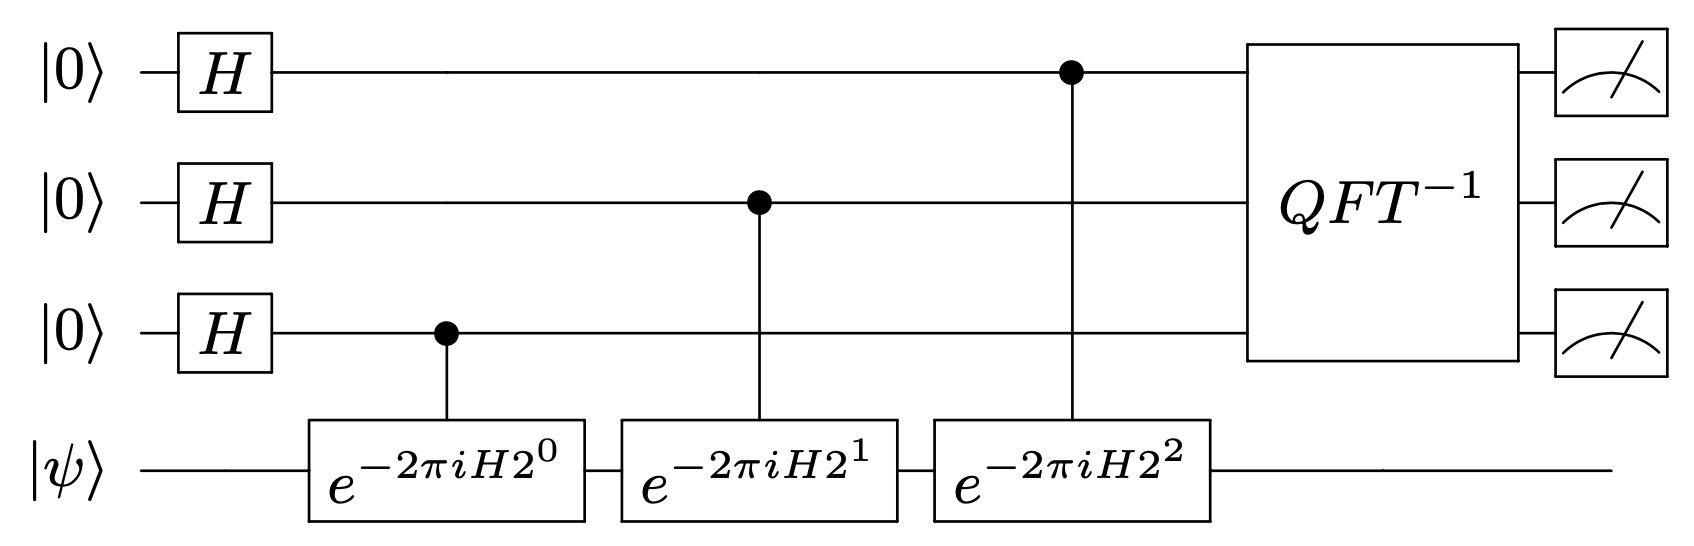
\includegraphics[width=3.25in]{qpe.jpg}
\caption{The circuit for quantum phase estimation with time evolution using 3 ancilla qubits}
\label{qpe-cir}
\end{figure}

The application of phase estimation on the near-term quantum devices, with less than 100 qubits and shallow circuits, are limited in the foreseeable future, because it requires a large overhead of ancilla qubits to achieve a acceptable precision, gate with high-fidelity as well as long coherence time to get a asymptotic approximation of the exact dynamics. 


\subsection{Variational quantum eigensolver (VQE)}
For the NISQ era, a possible and promising alternative is to use hybrid quantum-classical algorithm, such as the variational quantum eigensolver,\cite{Peruzzo:2014kca,yung:2014,McClean:2015bs}
\begin{figure}[h!]
\centering
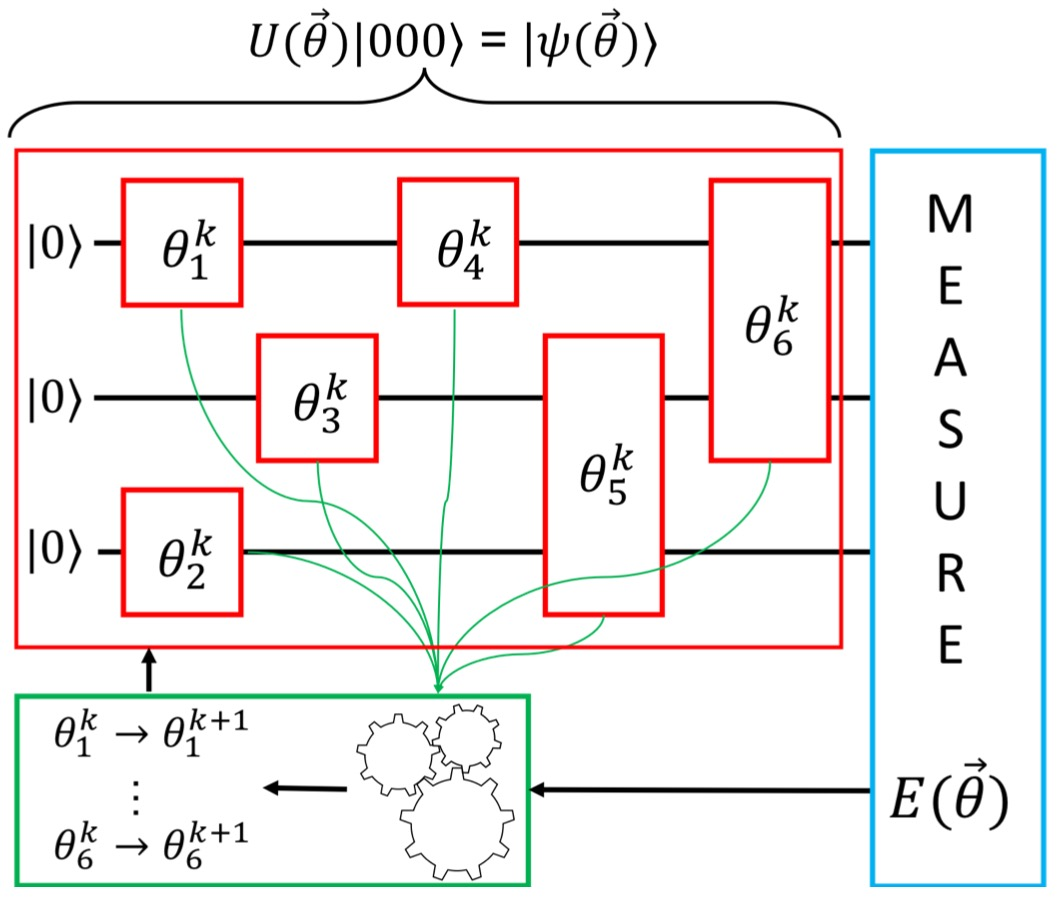
\includegraphics[width=2.0in]{vqe.jpg}
\caption{The schematic of the variational quantum eigensolver (VQE) for 3 qubits}
\label{vqe-cir}
\end{figure}
which only uses the quantum computer for storing and measuring the wavefunction, the classically intractable part. This variational scheme trades a large but polynomial overhead of measurements and classical optimization for the shorter coherence time.

Figure \ref{vqe-cir} shows the mechanism of a working VQE algorithm. A small quantum computer is employed to prepare a state (red) and to read out energies (blue), which will go to a classical optimization subroutine together with the current set of parameters. The classical computer (green) performs the minimization of the energy and updates parameters. Then, the new parameters are fed back into the quantum circuit. The whole process iterates until the energy converges.


%\newpage
\bibliographystyle{achemso}
\bibliography{report.bib}{}

\end{document}